% Created 2016-05-07 Sat 17:16
\documentclass[9pt,b5paper]{article}
\usepackage{fontspec}
\setmainfont{STSong} 
\usepackage{graphicx}
\usepackage{xcolor}
\usepackage{xeCJK}
\setCJKmainfont{STSong}
\usepackage{longtable}
\usepackage{float}
\usepackage{textcomp}
\usepackage{geometry}
\geometry{left=0cm,right=0cm,top=0cm,bottom=0cm}
\usepackage{multirow}
\usepackage{multicol}
\usepackage{listings}
\usepackage{algorithm}
\usepackage{algorithmic}
\usepackage{latexsym}
\usepackage{natbib}
\usepackage[xetex,colorlinks=true,CJKbookmarks=true,linkcolor=blue,urlcolor=blue,menucolor=blue]{hyperref}


\lstset{language=c++,numbers=left,numberstyle=\tiny,basicstyle=\ttfamily\small,tabsize=4,frame=none,escapeinside=``,extendedchars=false,keywordstyle=\color{blue!70},commentstyle=\color{red!55!green!55!blue!55!},rulesepcolor=\color{red!20!green!20!blue!20!}}
\author{deepwaterooo}
\date{\today}
\title{Java Programming Course Project Spring 2016}
\hypersetup{
  pdfkeywords={},
  pdfsubject={},
  pdfcreator={Emacs 24.5.1 (Org mode 8.2.7c)}}
\begin{document}

\maketitle
\tableofcontents


\section{Cube}
\label{sec-1}
\begin{itemize}
\item music is back once Renderer's OnSurfacePickedListener was set properly.
\item but due to lack of rest, I am so sick of the mediaplayer states now. Will work on 3d tetris implementation in the evening after some rest, and come back to work on this one some other time when my mind is clear.
\item Game flow through, debugging, onpick listener back now, needs to get my music back. nothing difficult, should be able to finish soon. understands the listener, adapter thing much better than DrawingFun periods. working on it now, Will update when finished.
\item A lightweighted mediaplayer referenced from online to correct my weired way of coding for Android MediaPlayer.
\item took all the effort to make MyGLSurfaceView working with an seekbar. But I may still need a couple of hours to fix the rest minor bugs. But it worth trying for such a MediaPlayer for videos, as well as for correcting my MediaPlayer coding style.
\item got too tired today, especially in the late evening hours, don't want to work on it any more, but will work on it tomorrow without status reports, but will commit a relative-final version.
\item It has been a long day, good night, my beloved cousin\textasciitilde{}! good night online surfers. How am I going to pay my summer tuition fees?  God, I need a job so badly\ldots{}\ldots{}
\item 
\item I am not proud of implementing multiple textures cause it's nothing original, but I feel happy that I could implement my app the way I originally wanted without cutting any features out, and building my confidence that as far as I want, I can find the way and do (/implement) it.
\item Todos: for following several hours, 
\begin{itemize}
\item I may work on tune and fine the app to make the music I like, for examples the songs that I loved, "waiting for you", "(Everything I Do) I Do It For You (my beloved cousin)" etc.
\item Tomorrow once this one is done, I will focus on opengl 3d tetris, accompany with unity CA \&\& WA elements building for practice (mainly through watching youtube videos).
\end{itemize}
\item The reason for choosing pictures: 
\begin{itemize}
\item horse: my beloved cousin's birth year;
\item sheep: my birth year;
\item dog: my cousin has a dog, and I have a dog at home too, they should hang out sometime, while my cousin and I need to stay together.
\item rabbit: my cousin and I both love this one a lot.
\item butterfly: It suffers and eventually it becomes a beautiful butterfly\textasciitilde{}!
\end{itemize}
\item Tetris theme music played by MediaPlayer can only function as the background music now.
\item Emacs + Auctex + org-mode can only export english correct with source codes, but can NOT export Chinese correctly from tex file yet. Need to find out the correct way to enable various kinds of latex engines from Auctex emacs mode.
\end{itemize}
\subsection{May Love Last Forever}
\label{sec-1-1}
\begin{itemize}
\item Please don't get anything wrong, I always love my cousin, and as I can NOT make it any more clearer: \textbf{I will be right here in CA waiting for you.}
\end{itemize}

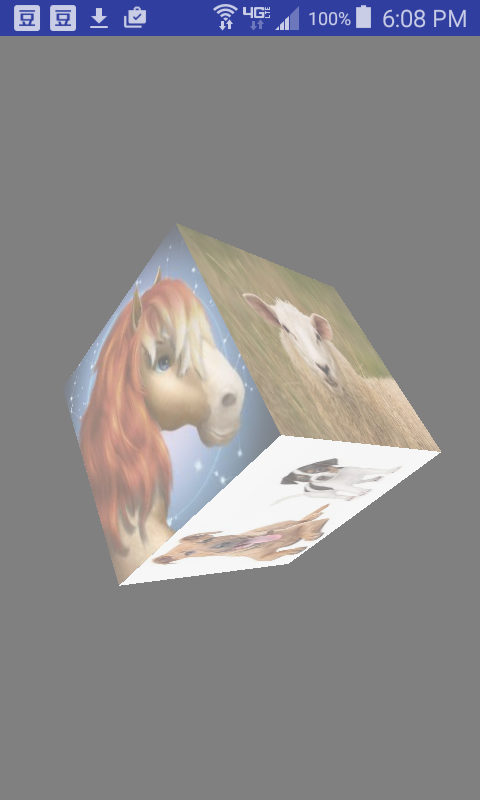
\includegraphics[width=.9\linewidth]{./Screenshot_2016-05-06-18-08-06.png}
\begin{itemize}
\item updated version of screen record vedio without music was put at \url{https://www.youtube.com/watch?v=3fxbz2jUFE4} or by search \textbf{deepwaterooo wang} \url{https://www.youtube.com/results?search_query=deepwaterooo+wang}
\item Current starting point turnning cube video was put at \url{https://www.youtube.com/watch?v=EuILt6B0YS0}
\end{itemize}

\section{References}
\label{sec-2}
\subsection{music: online \& local}
\label{sec-2-1}
\begin{itemize}
\item \url{http://www.cnblogs.com/xiaoQLu/archive/2011/04/24/2026520.html}
\item 生命周期 \url{http://wangzhaoli.blog.51cto.com/7607113/1290206}
\item \url{http://lpqsun-126-com.iteye.com/blog/1095108}
\item video \url{https://www.youtube.com/watch?v=LKL-efbiIAM}
\item mediaplayer 音频: \url{http://blog.csdn.net/siyehuazhilian/article/details/17111265}
\item 视频:\url{http://blog.csdn.net/lonelyroamer/article/details/7484297}
\item Seekbar \url{http://blog.csdn.net/hellogv/article/details/5975864}
\item customize seekbar: \url{http://stackoverflow.com/questions/16163215/android-styling-seek-bar}
\item surfaceview mediaplayer详解 \url{http://www.cnblogs.com/plokmju/p/android_SurfaceView.html}
\item \url{http://itfish.net/article/56684.html}
\item \url{http://blog.csdn.net/flyingfox023/article/details/18826597}
\item \url{http://www.voidcn.com/blog/womengmengyan/article/p-4537709.html}
\item 三阶魔方 \url{http://wenku.baidu.com/view/6e7b0d22915f804d2b16c1c1.html}
\item \url{http://www.yanhao.site/2015/10/29/Android\%E4\%B8\%AD\%E4\%B8\%BA\%E4\%BA\%8B\%E4\%BB\%B6\%E7\%BB\%91\%E5\%AE\%9A\%E7\%9B\%91\%E5\%90\%AC\%E5\%99\%A8\%E7\%9A\%84\%E5\%87\%A0\%E7\%A7\%8D\%E6\%96\%B9\%E6\%B3\%95/}
\item mp4文件格式解析 \url{http://blog.sina.com.cn/s/blog_48f93b530100jz4x.html}
\item 
\item 
\item 
\item 
\item 
\item 
\item 
\item 
\item Cube DJ for Android: \url{https://www.youtube.com/watch?v=vew7M-IOWHM}
\item PK Music Player Bass Bosster (may need as a References) \url{http://m.aptoide.com/app/com.paykerstudio.musicplayer/pk-music-player-bass-bosster?lang=zh}
\end{itemize}
\subsection{Textures}
\label{sec-2-2}
\begin{itemize}
\item cube map: \url{http://www.guidebee.info/wordpress/archives/3012}
\item cubemaps: \url{http://learnopengl.com/#!Advanced-OpenGL/Cubemaps}
\item compressed textures \url{http://www.guidebee.info/wordpress/archives/2988}
\item GLES20 \url{http://blog.csdn.net/liyuanjinglyj/article/details/46670819}
\item \url{http://www.zwqxin.com/archives/opengl/learn-texture-array.html}
\item \url{https://www.youtube.com/watch?v=jK6sfbw5oYQ}
\item 立方体纹理(cube map)概念 \url{http://www.bagualu.net/wordpress/archives/2405#d纹理-1} 
  有两种自动生成模式GL$_{\text{REFLECTION}}$$_{\text{MAP}}$ 和 GL$_{\text{NORMAL}}$$_{\text{MAP.}}$
\item OpenGL原理介绍 \url{http://www.twinklingstar.cn/2015/1532/introduce-to-opengl/}
\item Multitexturing \url{http://www.clockworkcoders.com/oglsl/tutorial8.htm}
\item 6 textures 立方体 \url{https://www.youtube.com/watch?v=rpq8aNKNLxA}
\item \url{http://www.zenlife.tk/an-intro-to-modern-opengl-2-3.md}
\end{itemize}
\subsection{previous}
\label{sec-2-3}
\begin{itemize}
\item c++: \url{http://blog.sina.com.cn/s/blog_b932048b0101fglx.html}
\item gl10: \url{http://blog.csdn.net/wangkuifeng0118/article/details/7425029}
\item ideas: \url{http://www.boyunjian.com/do/article/snapshot.do?uid=4560684719895433921}
\item gl10 with threads \url{http://www.cnblogs.com/carmanloneliness/archive/2012/01/06/2314909.html}
\item src: \url{http://vaero.blog.51cto.com/4350852/790620}
\item src: \url{http://vaero.blog.51cto.com/4350852/790637}
\item youtube videoes: \url{https://www.youtube.com/watch?v=hpnd11doMgc}
\item youtube videoes:\url{https://www.youtube.com/watch?v=3yLL9ADo-ko}
\item raypick: \url{https://github.com/76260865/OpenGLSETest}
\item trial: \url{http://www.j2megame.com/html/xwzx/ty/1416.html}
\item trial: \url{https://github.com/MediaMonks/tilt-game-android/blob/master/sensorlib/src/main/java/org/hitlabnz/sensor_fusion_demo/representation/Vector3f.java}
\item push pop matrix: \url{http://www.cnblogs.com/bhlsheji/p/4058745.html}
\item glPerspective \url{http://blog.csdn.net/popy007/article/details/1797121}
\item 拾取 \url{http://www.docin.com.cn/p-231068818.html}
\item 拾取精确 \url{http://www.docin.com.cn/p-223688481.html}
\item 豆丁: glPickMatrix \url{http://www.docin.com.cn/p-219126610.html}
\item glOrtho() Matrix \url{http://www.docin.com.cn/p-1541079192.html}
\item \url{http://www.docin.com.cn/p-1449786833.html}
\item 齐次坐标系: \url{http://www.docin.com.cn/p-200902035.html}
\item 可逆矩阵和求逆矩阵的方法 \url{http://www.docin.com.cn/p-102655207.html}
\item Direct3D中实现图无的鼠标拾取 \url{http://www.docin.com.cn/p-25415158.html}
\item 一个简单的OpenGL拾取例子 \url{http://itdocument.com/228389737/}
\item video Android 3D游戏开发(高级篇)--Opengl ES游戏引擎实现 \url{http://www.hztraining.com/bbs/showtopic-120.aspx}
\item 豆丁\url{http://116.213.76.141/search.do?nkey=android+3d+\%E6\%B8\%B8\%E6\%88\%8F+\%E5\%BC\%80\%E5\%8F\%91+\%E5\%9F\%BA\%E7\%A1\%80+\%E7\%AC\%AC27\%E8\%AF\%BE-\%E5\%B0\%84\%E7\%BA\%BF\%E6\%8B\%BE\%E5\%8F\%96&searchcat=1002&from=end&mode=4}
\item examples \url{http://www.docin.com/p-390492547.html}
\item MVPW \url{http://www.docin.com/p-909145095.html}
\item gluLookAt \url{http://blog.csdn.net/wangdingqiaoit/article/details/39433141} 与实现方法相同
\item work on camera \url{http://blog.csdn.net/wangdingqiaoit/article/details/39937019}
\item 纹理贴图: \url{http://wenku.baidu.com/view/b7d4c2dc5022aaea998f0f61.html}
\item 颜色材质与纹理映射 \url{http://202.114.108.237/Download/8a712530-bc61-4990-a86f-9ddd3300bf9d.pdf}
\item 视差贴图(Parallax Mapping) 难 \url{http://learnopengl-cn.readthedocs.io/zh/latest/05\%20Advanced\%20Lighting/05\%20Parallax\%20Mapping/}
\item textures: \url{http://blog.csdn.net/ypist/article/details/8603077}
\item music cube: \url{https://www.youtube.com/watch?v=FJUq_gWHTbI}
\item mediaplayer: \url{http://stackoverflow.com/questions/30881722/media-player-error-19-0}
\item fundamental: perspective othorgonal \url{https://www.youtube.com/watch?v=BgIsTZiyvvU}
\item music: \url{https://www.youtube.com/watch?v=N_Lpe_9VD2A&index=7&list=PLbmEQyKwSKqKX8R0vyRkZxgsZskw6SKcS}
\item three together: \url{https://www.youtube.com/watch?v=YqiArMjtXyE}
\item primitive textures: \url{https://www.youtube.com/watch?v=jgzTLXwsXP0}
\item marching cubes: \url{https://www.youtube.com/watch?v=ObmHOxeoIdw}
\item 程序园 \url{http://www.voidcn.com/blog/mapdigit/cata/1144071/}
\end{itemize}
% Emacs 24.5.1 (Org mode 8.2.7c)
\end{document}